\begin{explanationbox}
\textbf{一、为什么两项不再互相抵消增长？} 以 $f(x)=x-1/x$ 为例：
\[
\begin{array}{c|rrrrrr}x&-2&-1&-1/2&1/2&1&2\\\hline f(x)&-3/2&0&3/2&-3/2&0&3/2\end{array}
\]
在同一支上，$x$ 增大时，$x$ 增大，$-1/x$ 也增大，所以总和严格增大。与对勾函数不同，两项的变化方向一致。
\begin{center}
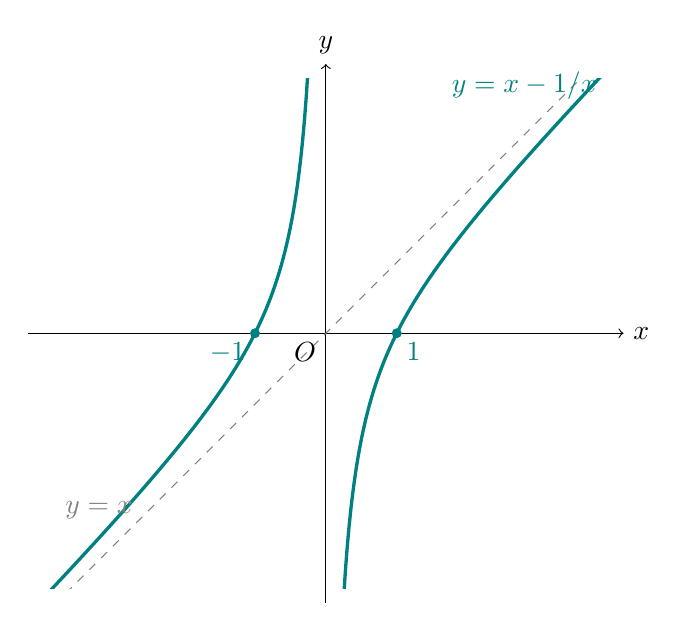
\begin{tikzpicture}[scale=0.9]
\draw[->] (-4.2,0)--(4.2,0) node[right] {$x$};
\draw[->] (0,-3.8)--(0,3.8) node[above] {$y$};
\begin{scope}
\clip (-4,-3.6) rectangle (4,3.6);
\draw[dashed,gray] (-4,-4)--(4,4);
\draw[teal,very thick,domain=-4:-0.25,samples=150] plot (\x,{\x-1/\x});
\draw[teal,very thick,domain=0.25:4,samples=150] plot (\x,{\x-1/\x});
\end{scope}
\fill[teal] (-1,0) circle (2pt) node[below left] {$-1$};
\fill[teal] (1,0) circle (2pt) node[below right] {$1$};
\node[teal] at (2.8,3.5) {$y=x-1/x$};
\node[gray] at (-3.2,-2.5) {$y=x$};
\node[below left] at (0,0) {$O$};
\end{tikzpicture}
\end{center}

\textbf{二、为什么中间没有值域空缺？} 正半轴靠近零时，$-B/x$ 可以任意小；向右走时 $Ax$ 可以任意大。负半轴由原点对称得到同样的值域。完整的取值证明见方法三。

\textbf{三、图像与直线的关系。} $f(x)-Ax=-B/x$：正半轴图像在 $y=Ax$ 下方，负半轴在其上方；横坐标绝对值越大，竖直差的绝对值越小。

\textbf{四、同一高度的两点。} 给定高度 $c$，两个横坐标由同一个二次方程得到；它们的乘积不随高度改变。这比单纯记住图形更有用。
\end{explanationbox}
